\section{Extension to Multiple Categories}

We present here how the methodology described in Section~\ref{inference_methodology} for
two categories can be extended to multiple categories.
To this end, we separate the income values into five distinct groups $ H_1, \ldots, H_5 \subseteq G$ of increasing wealth where:
\[
	g \in H_i \iff g_s \in R_i
\]
and the income ranges are set as follows (in Mexican pesos):
\begin{align*}
	R_1 &= \left[1000, 2500\right) \\
	R_2 &= \left[2500, 7500\right) \\
	R_3 &= \left[7500, 20000\right) \\
	R_4 &= \left[20000, 50000\right) \\
	R_5 &= \left[50000, \infty\right). \\
\end{align*}

Again, we define the set $Q$ as the group of users having at least one connection link to bank clients. For each user $q^j \in Q$, we compute the number of outgoing calls $a^j_i$ to the category $H_i$. 
We use the amount of calls $a^j_i$  as parameters defining a Dirichlet distribution for the probability of belonging to a given category. 
We define below the Dirichlet probability distribution function $D^j$:  

\begin{equation}
D^j \left( x_1, \ldots, x_5; \alpha^j_1, \ldots, \alpha^j_5 \right) = \frac{1}{\Beta \left( \alpha \right)} \prod^5_{i = 1} x_i^{\alpha^j_i - 1}
\label{Dirichlet}
\end{equation}

Where $\alpha^j_i = a^j_i +1$, are the parameters of the Dirichlet distribution, and $\Beta$ is the multivariate beta distribution function, defined according to: % (\eqref{Beta})

\begin{equation}
\Beta \left( \alpha_1, \ldots, \alpha_k \right) = \frac{\prod^k_{i = 1} \Gamma \! \left( \alpha_i \right)}{\Gamma \! \left( \sum^k_{i = 1} \alpha_i \right) }
\label{Beta} 
\end{equation}

Note that the above equation defines a distinct Dirichlet distribution for each user. For each one of these distributions we computed the marginal probability functions across all different categories, which results in a $Beta$ distributed functions, and use its to get the  lowest 5 percentiles ($p_{lower_{i}}$) in each case ${i=1, \ldots 5}$ which can be compared to assign a category to each user. 

In order to gain intuition on how this approach extends to the multiple category case we constructed for each category $i$ a binary classifier by using the computed $p_{lower_{i}}$ score and a given threshold $\tau$. In each case we slide the threshold $\tau$ and compute the resulting ROC curves as we shown in figure \ref{roc_multiple_categories}.

\begin{figure}
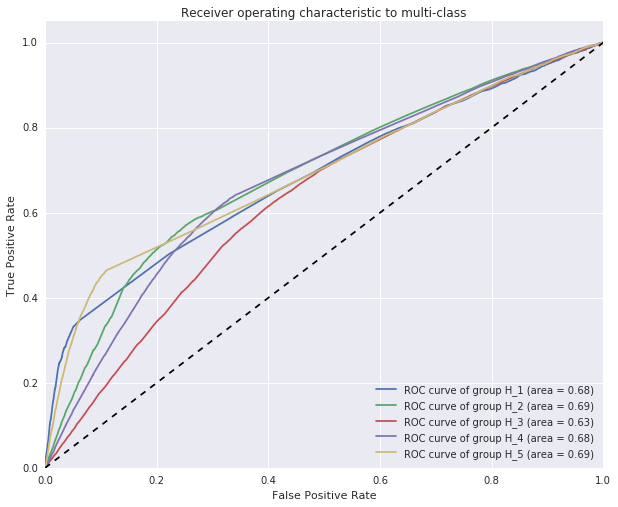
\includegraphics[width=\columnwidth]{figures/ROC_multiclass/ROC_multiclass.png}
\caption{ROC curve for multiclass problem. We observed different performances regarding to different categories: $AUC_1=0.68$, $AUC_2=0.69$,$AUC_3=0.63$,$AUC_4=0.68$,$AUC_5=0.69$. Again, these predictor imporove the random case and perform on a similar way (with exception of category 4)}
\label{roc_multiple_categories}
\end{figure}

It is worth of mention that the predictor with lower performance (category 4,$AUC=0.63$, income range $[7500,20000]$) matches cualitatively with the range were dispersion in the heatmap get broader (see figure \ref{homophily_heatmap}). This suggest that for this range of income it would be useful to complement the proposed approach with other orthogonal income information or prediction strategies, as users geolocalization, credit card debts, etc.  
%We use the Dirichlet distribution to define the following algorithm to infer the appropriate income category for each user 
